\section{Presentazione} \label{pres}
\begin{figure}[H]
\centering
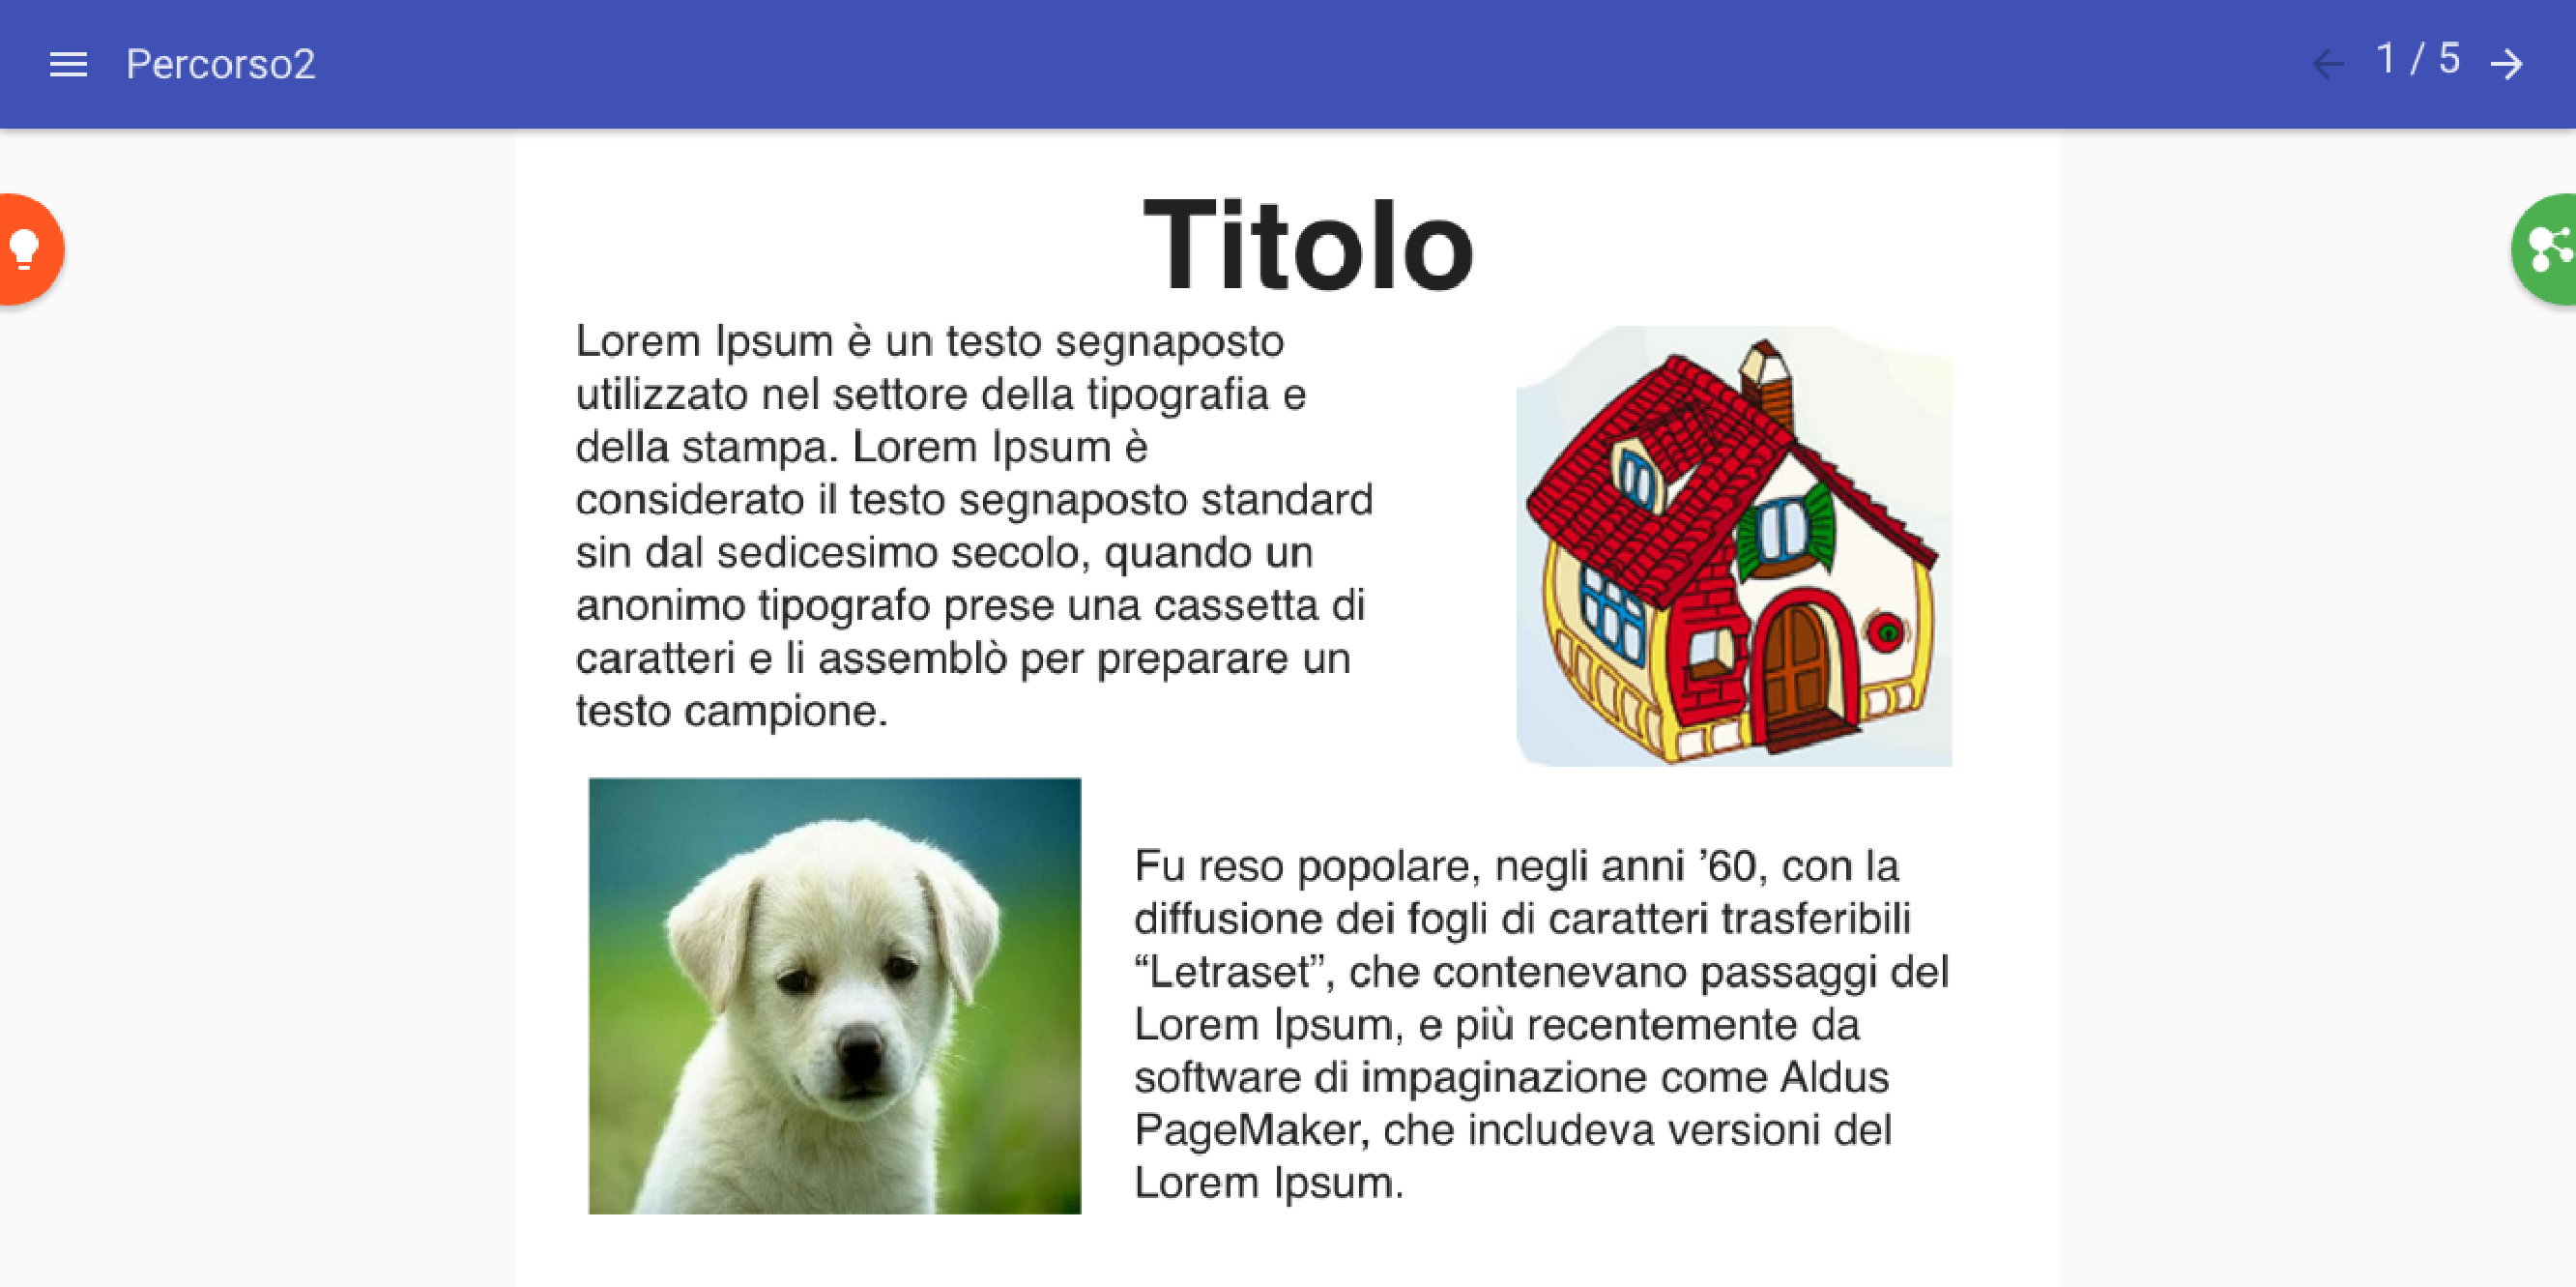
\includegraphics[scale=0.32]{immagini/presentazione.pdf}
\caption{Vista di presentazione}
\end{figure}
Questa pagina è dedicata all'esecuzione di presentazione, cioè la visualizzazione ordinata di una sequenza di \gloxy{frame}.\\
L'utente può accedere a questa pagina dopo aver selezionato un \gloxy{progetto}, scelto un \gloxy{percorso di presentazione} personalizzato e aver selezionato l'avvio della presentazione. \\
La presentazione viene generata utilizzando i \gloxy{frame} presenti all'interno dei nodi della mappa mentale, i quali verranno visualizzati secondo l'ordine stabilito dal \gloxy{percorso} di presentazione.
\subsection{Pannello di navigazione}
Gli strumenti principali che permette all'utente di spostarsi all'interno della presentazione sono \textbf{freccia a destra} 
\includegraphics[scale=0.5]{immagini/frecciaDestra.pdf} e \textbf{freccia a sinistra} 
\includegraphics[scale=0.5]{immagini/frecciaSinistra.pdf} che si trova in alto a destra nella vista di presentazione e i due menù laterali.
\begin{figure}[H]
\centering
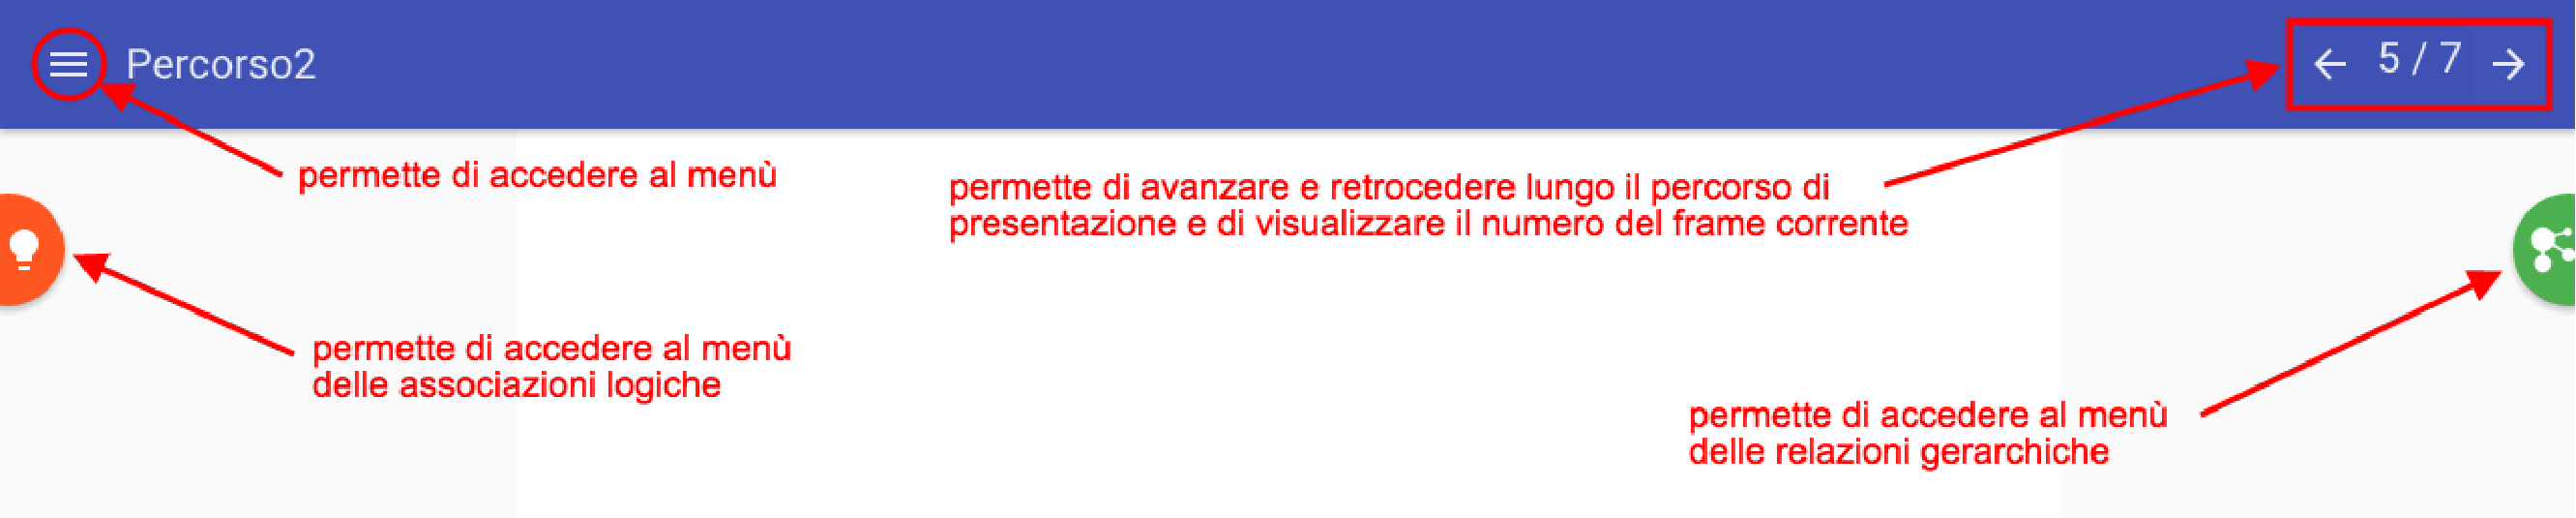
\includegraphics[scale=0.32]{immagini/imgFrecciePres.pdf}
\caption{Strumenti della vista di presentazione}
\end{figure}
\subsection{Menu laterali}
I due menu permettono all'utente di effettuare dei \textit{salti} dal \gloxy{frame} corrente ad un \gloxy{frame} ad esso correlato tramite relazione gerarchica o associazione logica.\\
Quando l'utente sta visualizzando un \textit{\gloxy{frame}} può passare alla visualizzazione di un altro \textit{\gloxy{frame}}, anche non appartenente al \gloxy{percorso} di presentazione, purché il nodo che lo contiene abbia un qualche tipo di relazione con quello corrente.
Una volta effettuato questo salto la presentazione passa in modalità ``\textit{non lineare}'', impedendo all'utente di cambiare \gloxy{frame} utilizzando le frecce.\\
Per riprendere la presentazione lineare e ritornare all'ultimo \gloxy{frame} del \gloxy{percorso} visualizzato è necessario premere l'apposito pulsante 
\includegraphics[scale=0.5]{immagini/frecciaRicurva.pdf} presente nel \textbf{\textit{Pannello di navigazione}}.
\subsubsection{Menu delle associazioni logiche}
\begin{figure}[H]
\centering
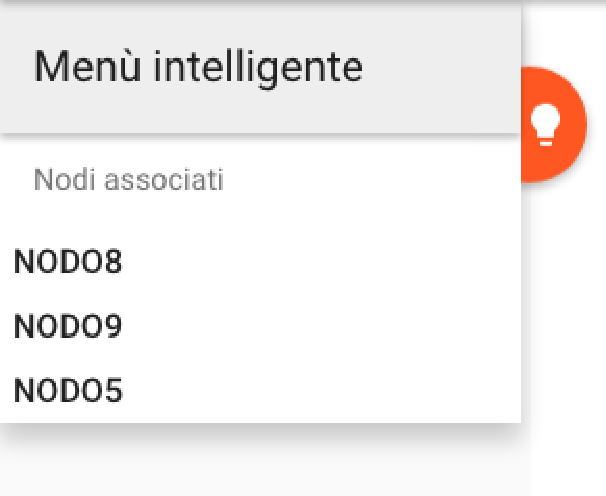
\includegraphics[scale=0.5]{immagini/menuLogico.pdf}
\caption{Menù delle associazioni logiche}
\end{figure}
Questo menu contiene una lista dei nodi della mappa mentale, collegati al nodo contenente il \gloxy{frame} corrente, tramite un'associazione logica.\\
L'utente può accedere a questo menù premendo l'etichetta a sinistra rappresentante una lampadina 
\includegraphics[scale=0.5]{immagini/lampadina.pdf}.\\
Selezionando uno dei nodi presenti all'interno di questo menu si andrà a visualizzare il \gloxy{frame} che contenuto in quel nodo, anche se il nodo non fa parte del \gloxy{percorso} di presentazione.
\subsubsection{Menu delle relazioni gerarchiche}
\begin{figure}[H]
\centering
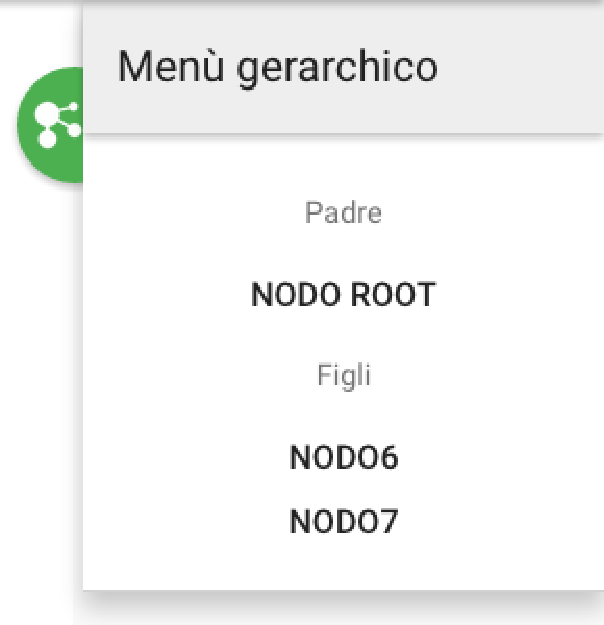
\includegraphics[scale=0.5]{immagini/menuGerarchico.pdf}
\caption{Menù delle relazioni gerarchiche}
\end{figure}
Questo menu contiene una lista dei nodi della mappa mentale, collegati al nodo contenente il \gloxy{frame} corrente tramite una relazione gerarchica.\\
L'utente può accedere a questo menù premendo l'etichetta a destra rappresentante un grafo 
\includegraphics[scale=0.5]{immagini/grafo.pdf} .\\
Selezionando uno dei nodi presenti all'interno di questo menu si andrà a visualizzare il \gloxy{frame} che rappresenta quel nodo, anche se il nodo non fa parte del \gloxy{percorso} di presentazione.
